\documentclass[10pt,a4paper]{article}
\usepackage[right=0.5cm, left=0.5cm,top=0.5cm,bottom=0.5cm]{geometry}
\usepackage{enumitem}
\usepackage{graphicx}
\usepackage{array, tasks}
\usepackage{blindtext}
\usepackage{fontspec}
\usepackage{amsmath,amsfonts,amssymb,mathrsfs,amsthm}
\usepackage{fancyhdr}
\usepackage{xcolor}
\usepackage{booktabs}
\usepackage[font={bf}]{caption}
% \captionsetup[table]{box=colorbox,boxcolor=orange!20}
\usepackage{float}
\usepackage{esvect}
\usepackage{tabularx}
\usepackage{pifont}
\usepackage{colortbl}
 \usepackage{fancybox}
 \mathversion{bold}
 \usepackage{pgfplots}
 % \usepackage[utf8]{inputenc}
\usepackage{tikz}
 \usepackage[tikz]{bclogo}%
 \usepackage{mathpazo}
\usepackage{ulem}
\usepackage{yagusylo}
\usepackage{textcomp}\usepackage{blindtext}
\usepackage{multicol}
\usepackage{varwidth}
\usetikzlibrary{calc,intersections}
\usepackage{pgfplots}
%\usepackage{fourier}
\pgfplotsset{compat=1.11}
\usepackage{tkz-tab}
\usepackage{xcolor}
\usepackage{color}
\usetikzlibrary{calc}
\mathchardef\times="2202
\usepackage[most]{tcolorbox}
\definecolor{lightgray}{gray}{0.9}
\definecolor{ocre}{RGB}{0,244,244} 
\definecolor{head}{RGB}{255,211,204}
\definecolor{browndark}{RGB}{105,79,56}
%\RequirePackage[framemethod=default]{mdframed}
\usepackage{tikz}
\usetikzlibrary{calc,patterns,decorations.pathmorphing,arrows.meta,decorations.markings}
\usetikzlibrary{arrows.meta}
\makeatletter
\tcbuselibrary{skins,breakable,xparse}
\tcbset{%
  save height/.code={%
    \tcbset{breakable}%
    \providecommand{#1}{2cm}%
    \def\tcb@split@start{%
      \tcb@breakat@init%
      \tcb@comp@h@page%
      \def\tcb@ch{%
        \tcbset{height=\tcb@h@page}%
        \tcbdimto#1{#1+\tcb@h@page-\tcb@natheight}%
        \immediate\write\@auxout{\string\gdef\string#1{#1}}%
        \tcb@ch%
      }%
      \tcb@drawcolorbox@standalone%
    }%
  }%
}
\newcommand{\Lim}{\displaystyle\lim}
\makeatother
\newcommand{\oij}{$\left( \text{O};\vv{i},\vv{j} , \vv{k}\right)$}
\colorlet{darkred}{red!30!black}
\newcommand{\red}[1]{\textcolor{darkred}{ #1}}
\newcommand{\rr}{\mathbb{R}}
\renewcommand{\baselinestretch}{1.2}
 \setlength{\arrayrulewidth}{1.25pt}
\usepackage{titlesec}
\usepackage{titletoc}
\usepackage{minitoc}
\usepackage{ulem}
%--------------------------------------------------------------

\usetikzlibrary{decorations.pathmorphing}
\tcbuselibrary{skins}

%%%%%%%%%%%
%-------------------------------------------------------------------------
\tcbset{
        enhanced,
        colback=white,
        boxrule=0.1pt,
        colframe=brown!10,
        fonttitle=\bfseries
       }
\definecolor{problemblue}{RGB}{100,134,158}
\definecolor{idiomsgreen}{RGB}{0,162,0}
\definecolor{exercisebgblue}{RGB}{192,232,252}
\definecolor{darkbrown}{rgb}{0.4, 0.26, 0.13}

\newcommand*{\arraycolor}[1]{\protect\leavevmode\color{#1}}
\newcolumntype{A}{>{\columncolor{blue!50!white}}c}
\newcolumntype{B}{>{\columncolor{LightGoldenrod}}c}
\newcolumntype{C}{>{\columncolor{FireBrick!50}}c}
\newcolumntype{D}{>{\columncolor{Gray!42}}c}

\newcounter{mysection}
\newcounter{mysubsection}
\newcommand{\mysection}[1]{%
    \stepcounter{mysection} % Increment the counter
    \textcolor{red}{\LARGE\themysection. #1 :}
}
\newcommand{\mysubsection}[2]{
    \stepcounter{mysubsection}
    \textcolor{red}{\large \themysection.#1. #2 :}
}
% \textcolor{red}{\LARGE\bfseries 1. Les équation du deuxiéme degrée :}

%------------------------------------------------------
\newtcolorbox[auto counter]{Definition}{enhanced,
before skip=2mm,after skip=2mm,
colback=yellow!20!white,colframe=lime,boxrule=0.2mm,
attach boxed title to top left =
    {xshift=0.6cm,yshift*=1mm-\tcboxedtitleheight},
    varwidth boxed title*=-3cm,
    boxed title style={frame code={
                        \path[fill=lime]
                            ([yshift=-1mm,xshift=-1mm]frame.north west)  
                            arc[start angle=0,end angle=180,radius=1mm]
                            ([yshift=-1mm,xshift=1mm]frame.north east)
                            arc[start angle=180,end angle=0,radius=1mm];
                        \path[left color=lime,right color = lime,
                            middle color = lime]
                            ([xshift=-2mm]frame.north west) -- ([xshift=2mm]frame.north east)
                            [rounded corners=1mm]-- ([xshift=1mm,yshift=-1mm]frame.north east) 
                            -- (frame.south east) -- (frame.south west)
                            -- ([xshift=-1mm,yshift=-1mm]frame.north west)
                            [sharp corners]-- cycle;
                            },interior engine=empty,
                    },
fonttitle=\bfseries\sffamily,
title={Definition ~\thetcbcounter}}
%------------------------------------------------------
\newtcolorbox[auto counter]{Proposition}{enhanced,
before skip=2mm,after skip=2mm,
colback=yellow!20!white,colframe=blue,boxrule=0.2mm,
attach boxed title to top left =
    {xshift=0.6cm,yshift*=1mm-\tcboxedtitleheight},
    varwidth boxed title*=-3cm,
    boxed title style={frame code={
                        \path[fill=blue]
                            ([yshift=-1mm,xshift=-1mm]frame.north west)  
                            arc[start angle=0,end angle=180,radius=1mm]
                            ([yshift=-1mm,xshift=1mm]frame.north east)
                            arc[start angle=180,end angle=0,radius=1mm];
                        \path[left color=blue,right color = blue,
                            middle color = blue]
                            ([xshift=-2mm]frame.north west) -- ([xshift=2mm]frame.north east)
                            [rounded corners=1mm]-- ([xshift=1mm,yshift=-1mm]frame.north east) 
                            -- (frame.south east) -- (frame.south west)
                            -- ([xshift=-1mm,yshift=-1mm]frame.north west)
                            [sharp corners]-- cycle;
                            },interior engine=empty,
                    },
fonttitle=\bfseries\sffamily,
title={Proposition ~\thetcbcounter}}
%------------------------------------------------------
\newtcolorbox[auto counter]{Thm}[1]{enhanced,
before skip=2mm,after skip=2mm,
colback=yellow!20!white,colframe=red,boxrule=0.2mm,
attach boxed title to top left =
    {xshift=0.6cm,yshift*=1mm-\tcboxedtitleheight},
    varwidth boxed title*=-3cm,
    boxed title style={frame code={
                        \path[fill=red]
                            ([yshift=-1mm,xshift=-1mm]frame.north west)  
                            arc[start angle=0,end angle=180,radius=1mm]
                            ([yshift=-1mm,xshift=1mm]frame.north east)
                            arc[start angle=180,end angle=0,radius=1mm];
                        \path[left color=red,right color = red,
                            middle color = red]
                            ([xshift=-2mm]frame.north west) -- ([xshift=2mm]frame.north east)
                            [rounded corners=1mm]-- ([xshift=1mm,yshift=-1mm]frame.north east) 
                            -- (frame.south east) -- (frame.south west)
                            -- ([xshift=-1mm,yshift=-1mm]frame.north west)
                            [sharp corners]-- cycle;
                            },interior engine=empty,
                    },
fonttitle=\bfseries\sffamily,
title={#1 ~\thetcbcounter}}
%------------------------------------------------------
\newtcolorbox[auto counter]{exemple}{
  % breakable,
  enhanced,
  colback=white,
  boxrule=0pt,
  arc=0pt,
  outer arc=0pt,
  title=Exemple ~\thetcbcounter,
  fonttitle=\bfseries\sffamily\large\strut,
  coltitle=problemblue,
  colbacktitle=problemblue,
  title style={
left color=exercisebgblue,
    right color=white,
    middle color=exercisebgblue  
  },
  overlay={
    \draw[line width=1pt,problemblue] (frame.south west) -- (frame.south east);
    \draw[line width=1pt,problemblue] (frame.north west) -- (frame.north east);
    \draw[line width=1pt,problemblue] (frame.south west) -- (frame.north west);
    \draw[line width=1pt,problemblue] (frame.south east) -- (frame.north east);
  }
}
%----------------------------------------------------
\newtcolorbox[auto counter]{application}{
  % breakable,
  enhanced,
  colback=white,
  boxrule=0pt,
  arc=0pt,
  outer arc=0pt,
  title=Application ~\thetcbcounter,
  fonttitle=\bfseries\sffamily\large\strut,
  coltitle=problemblue,
  colbacktitle=problemblue,
  title style={
left color=exercisebgblue,
    right color=white,
    middle color=exercisebgblue  
  },
  overlay={
    \draw[line width=1pt,problemblue] (frame.south west) -- (frame.south east);
    \draw[line width=1pt,problemblue] (frame.north west) -- (frame.north east);
    \draw[line width=1pt,problemblue] (frame.south west) -- (frame.north west);
    \draw[line width=1pt,problemblue] (frame.south east) -- (frame.north east);
  }
}
%----------------------------------------------------
\newtcolorbox[auto counter]{Activite}{
  % breakable,
  enhanced,
  colback=white,
  boxrule=0pt,
  arc=0pt,
  outer arc=0pt,
  title=Activité ~\thetcbcounter,
  fonttitle=\bfseries\sffamily\large\strut,
  coltitle=problemblue,
  colbacktitle=problemblue,
  title style={
left color=yellow!50!white,
    right color=white,
    middle color=yellow!20!white  
  },
  overlay={
    \draw[line width=1pt,problemblue] (frame.south west) -- (frame.south east);
    \draw[line width=1pt,problemblue] (frame.north west) -- (frame.north east);
    \draw[line width=1pt,problemblue] (frame.south west) -- (frame.north west);
    \draw[line width=1pt,problemblue] (frame.south east) -- (frame.north east);
  }
}
%---------------------------------------------
\newtcolorbox{mybox}[2]{enhanced,breakable,
    before skip=2mm,after skip=2mm,
    colback=white,colframe=#2!30!blue,boxrule=0.3mm,rightrule=0.3mm,
    attach boxed title to top center={xshift=0cm,yshift*=1mm-\tcboxedtitleheight},
    varwidth boxed title*=-3cm,
    boxed title style={frame code={
    \path[fill=#2!30!black]
    ([yshift=-1mm,xshift=-1mm]frame.north west)
    arc[start angle=0,end angle=180,radius=1mm]
    ([yshift=-1mm,xshift=1mm]frame.north east)
    arc[start angle=180,end angle=0,radius=1mm];
    \path[draw=black,line width=1pt,left color=#2!1!white,right color=#2!1!blue!65,
    middle color=#2!1!green]
    ([xshift=-2mm]frame.north west) -- ([xshift=2mm]frame.north east)
    [rounded corners=1mm]-- ([xshift=1mm,yshift=-1mm]frame.north east)
    -- (frame.south east) -- (frame.south west)
    -- ([xshift=-1mm,yshift=-1mm]frame.north west)
    [sharp corners]-- cycle;
    },interior engine=empty,
    },
title=#1,coltitle=black,fonttitle=\sffamily}
%---------------------------------------------
\newtcolorbox{boxone}{%
    enhanced,
    colback=brown!10,
    boxrule=0pt,
    sharp corners,
    drop lifted shadow,
    frame hidden,
    fontupper=\bfseries,
    notitle,
    overlay={%
        \draw[Circle-Circle, brown!70!black, line width=2pt](frame.north west)--(frame.south west); 
        \draw[Circle-Circle, brown!70!black, line width=2pt](frame.north east)--(frame.south east);}
    }
    
\begin{document}

\begin{tcolorbox}[title=\textcolor{blue}{\shadowbox{ Prof : Othmane Laksoumi}}
\hfill
\textcolor{blue}{\shadowbox{ Limites et continuité }}]

\end{tcolorbox}

\begin{mybox}{Lycée Qualifiant Zitoun}{gray}
    \begin{minipage}{8cm}
    \textcolor{darkbrown}{Année scolaire : } 2024-2025 \\
    \textcolor{darkbrown}{Niveau : } 2 Bac Sciences Physiques \\
    \textcolor{darkbrown}{Durée totale : } $15h$
    \end{minipage}
\end{mybox}

\begin{boxone}
{\Large\ding{45}}
\textcolor{red}{\large Contenus du programme :}
\begin{itemize}
    \item Continuité en un point ; continuité à droite ; continuité à gauche ; continuité sur un intervalle (cas de fonctions polynômes ; de fonctions rationnelles ; de fonctions trigonométriques et de la fonction \(x \mapsto \sqrt{x}\)).
    
    \item Image d'un intervalle et d'un segment par une fonction continue;
    \item Théorème des valeurs intermédiaires; cas d'une fonction continue et strictement monotone sur un intervalle.
    \item Fonction réciproque d'une fonction continue et strictement monotone sur un intervalle.
\end{itemize}

{\Large\ding{45}}
\textcolor{red}{\large Les capacités attendues :}
\begin{itemize}
    \item Déterminer l'image d'un segment ou d'un intervalle :
        \begin{itemize}
            \item Par une fonction continue.
            \item Par une fonction continue et strictement monotone.
        \end{itemize}
     \item Appliquer le théorème des valeurs intermédiaires pour l'étude de quelques équations ou inéquations ou pour l'étude du signe de quelques expressions ...
     \item Utiliser la dichotomie pour déterminer des valeurs approchées des solutions de l'équation $f(x) = \lambda$ ou pour encadrer ces solutions.
     \item Applique le théorème des valeurs intermédiaires et le théorème de la fonction réciproque dans le cas d'une fonction continue et strictement monotone sur un intervalle.
\end{itemize}

{\Large\ding{45}}
\textcolor{red}{\large Recommandations pédagogiques :} 
  \begin{itemize}
     \item On adoptera la définition suivante : « \(f\) est continue en \(x_0\) si \(\Lim_{x \to x_0} f(x) = f(x_0)\) ».
        \item On admettra les résultats concernant la continuité des fonctions polynômes, des fonctions rationnelles, des fonctions trigonométriques et de la fonction \(x \mapsto \sqrt{x}\), en mettant l'accent sur les applications de ces résultats.
      \item On admettra que que l'image d'un segment par une fonction continue est un segment ainsi que l'image d'un intervalle est un intervalle et aprés on en déduira le théorème des valeurs intermédiaires.
      \item On admettra que $f+g$ et $f\times g$ et $\lambda f$ sont des fonctions continues sur un intervalle $I$ si $f$ et $g$ sont continues sur $I$.
      \item On admettra que $g\circ f$ est une fonction continue sur un intervalle $I$ si $f$ est continue sur $I$ et $g$ est continue sur $f(I)$.
      
  \end{itemize}
\end{boxone}

\newpage

\begin{tabular}{|>{\raggedright\arraybackslash}p{17cm}|>{\centering\arraybackslash}p{0.8cm}|}
\hline
\rowcolor{head}

\centering Contenu du cour &
 Durée \\
\hline
 
\vspace{1mm}


\mysection{Continuité d'une fonction numérique} \newline
\mysubsection{1}{Continuité d'une fonction en un point}
\begin{Definition}
    Soit $f$ une fonction numérique definie sur un intervalle ouvert $I$ et $a\in I$. \\
    On dit que la fonction $f$ est continue au point $a$ si : $\Lim_{x\to a}f(x) = f(a)$.
\end{Definition}

\textcolor{red}{Interprétation graphique : }\newline
    \includegraphics[width=0.8\textwidth]{Capture.JPG}

\begin{exemple}
    \begin{enumerate}
        \item Soit $f$ la fonction numérique définie sur $\mathbb{R}$ par :
        $$\begin{cases}
            f(x) = \displaystyle\frac{x^2+x-6}{x-2} \hspace{3mm} \text{si } \ x\neq 2 \\
            f(2) = 5
        \end{cases}$$
        Montrons que la fonction $f$ est continue au point $a = 2$.
    \end{enumerate}
\end{exemple}

\begin{application}
    Dans chacun des cas suivants, étudier le continuité de la fonction $f$ au point $a$ :
    \begin{enumerate}
        \item $$\begin{cases}
            f(x) = \displaystyle\frac{\sin{x}}{x(\sqrt{x+1}-\sqrt{x})} \hspace{3mm} \text{si } \ x\neq 0\\
            f(0) = 1
        \end{cases} 
        \text{et } \ a = 0$$
        \item $$\begin{cases}
            f(x) = \displaystyle\frac{-2x^2-x+1}{x+1} \hspace{3mm} \text{si } \ x\neq -1 \\
            f(-1) = 1
        \end{cases} 
        \text{et } \ a = -1$$
    \end{enumerate}
\end{application}

\mysubsection{2}{Continuité à droite - continuité à gauche}
\begin{Definition}
    \begin{enumerate}
        \item Soit $f$ une fonction définie sur un intervalle de la forme $[a,a + \alpha[$ où $\alpha \in\mathbb{R}^*_+$. \\
        On dit que $f$ est \textcolor{red}{continue à droite} en $a$ si : 
        $\Lim_{x\to a^+}f(x) = f(a)$.
        \item Soit $f$ une fonction définie sur un intervalle de la forme $]a - \alpha,a]$ où $\alpha \in\mathbb{R}^*_+$. \\
        On dit que $f$ est \textcolor{red}{continue à gauche} en $a$ si : 
        $\Lim_{x\to a^-}f(x) = f(a)$.
    \end{enumerate}
\end{Definition} 

&
 \\
\hline

\end{tabular}

\newpage

\begin{tabular}{|>{\raggedright\arraybackslash}p{17cm}|>{\centering\arraybackslash}p{0.8cm}|}
\hline

\vspace{1mm}
\begin{exemple}
        Etudions la continuité à droite et à gauche des fonctions suivantes au point $a$ :
        $$\begin{cases}
            f(x) = 3-x^2 \hspace{3mm} \text{si } \ x\leq 0 \\ 
            f(x) = \displaystyle\frac{x^2-3}{2x-1} \hspace{3mm} \text{si } \ x> 0 \\
            a = 0
        \end{cases} \text{et} \begin{cases}
            g(x) = \displaystyle\frac{x^2-1}{|x-1|}  \text{si } \ x \neq 1\\
            g(1) = 2\\ 
            a = 1
        \end{cases}$$
\end{exemple}

\begin{Proposition}
    Une fonction numérique $f$ est continue au point $a$ si, et seulement si elle est continue à droite et à gauche au point $a$. En d'autres termes :
    $$(f \text{ continue au point $a$}) \Longleftrightarrow \Lim_{x\to a^-}f(x) = \Lim_{x\to a^+}f(x) = f(a)$$
\end{Proposition}
\begin{application}
    Dans chacun des cas suivants, étudier la continuité de la fonction $f$ au point $a$ : 
    \begin{enumerate}
        \item $$\begin{cases}
            f(x) = \displaystyle\frac{x^3-7x-6}{|x-3|}\hspace{3mm}\text{si } \ x\neq 3 \\
            f(3) = 20
        \end{cases}
        \text{ et } a = 3$$
        \item $$\begin{cases}
            f(x) = \displaystyle\frac{x^2+5x+6}{x^3+8} \hspace{3mm} \text{si } \ x>-2 \\ 
            f(x) = \displaystyle\frac{\sqrt{x+6} -2}{x+2} \hspace{3mm} \text{si } \ -6\leq x < -2 \\
            f(-2)=\displaystyle\frac{1}{4}
        \end{cases}
        \text{ et } a = -2$$
    \end{enumerate}
\end{application}

\mysubsection{3}{Continuité d'une fonction sur un intervalle}
\begin{Definition}
    \begin{enumerate}
        \item Une fonction $f$ est \textcolor{red}{continue sur un intervalle ouvert} $I$ si elle est continue en tout point de $I$.\\
        En particulier $f$ est continue sur $]a,b[$ si elle est continue en tout point de $]a,b[$.
        \item Une fonction $f$ est continue sur $[a,b]$ si elle est continue sur $]a,b[$ et continue à droite en $a$ et à gauche en $b$.
        \item Une fonction $f$ est continue sur $[a,b[$ si elle est continue sur $]a,b[$ et continue à droite en $a$.
        \item Une fonction $f$ est continue sur $]a,b]$ si elle est continue sur $]a,b[$ et continue à gauche en $b$.
    \end{enumerate}
\end{Definition}

\begin{Proposition}
    \begin{enumerate}
        \item Toute fonction constante est continue sur $\mathbb{R}.$
        \item Toute fonction polynomiale est continue sur $\mathbb{R}$.
        \item Toute fonction rationnelle est continue sur son domaine de définition.
        \item Les fonction $x\longmapsto \sin{x}$ et $x\longmapsto \cos{x}$ sont continues sur $\mathbb{R}$.
        \item la fonction $x\longmapsto \sqrt{x}$ est continue sur $\mathbb{R}^+$.
    \end{enumerate}
\end{Proposition}




&\\ 
\hline

\end{tabular}

\begin{tabular}{|>{\raggedright\arraybackslash}p{17cm}|>{\centering\arraybackslash}p{0.8cm}|}
\hline


\vspace{1mm}
\mysubsection{4}{Fonction partie entiére}
\begin{Activite}
    La fonction \textcolor{red}{partie entiére $E$} est définie sur $\mathbb{R}$ par $E(x) = n$, où $n$ est l'entier relatif tel que : $n\leq x < n+1$.\\
    Par exemple : $E(0.47) = 0$, $E(5.8) = 5$, $E(-0.4) = -1$.
    \begin{enumerate}
        \item Remplir le tableau suivant :\\
        \begin{tabular}{|c|c|c|c|c|c|c|}
        \hline
            $x$ & 3.5 & -5 & 1.23 & $\pi$ & $-\sqrt{2}$ & $\displaystyle\frac{5}{2}$\\ \hline
             $E(x)$ & &  & & & & \\ \hline
        \end{tabular}
        \item Que vaut $E(x)$ quand $x\in\mathbb{Z}$?
        \item Déterminer $E(x)$ pour tout $x\in [0,1[$ et pour tout $x\in [1,2[$.
        \item La fonction $E(x)$ est-elle continue en $1$?
    \end{enumerate}
\end{Activite}

\begin{Definition}
    Soit $x$ un nombre réel.\\
    \textcolor{red}{La partie entiére} de $x$ est le plus grand entier relatif $n$ qui est inférieur ou égal à $x$. On la \\note : $E(x)$. 
\end{Definition}

\textcolor{red}{Courbe représentative de la fonction partie entière :}
\vspace{-10mm}
\begin{center}
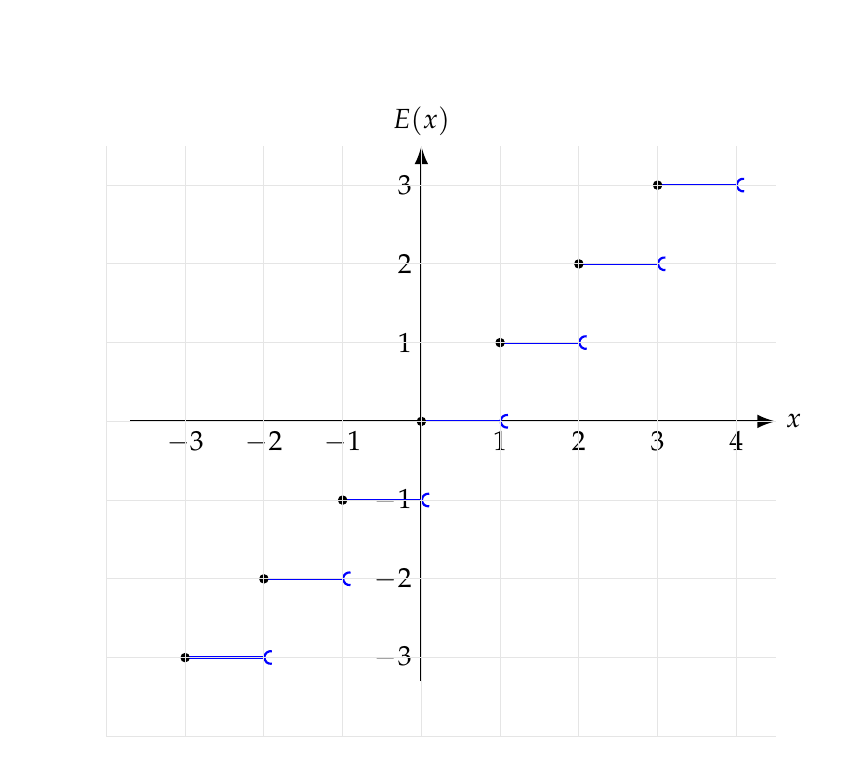
\begin{tikzpicture}
    % Draw axes
    \draw[-Latex, thick] (-3.7,0) -- (4.5,0) node[right] {$x$};
    \draw[-Latex, thick] (0,-3.3) -- (0,3.5) node[above] {$E(x)$};

    % Draw x-axis ticks and labels
    \foreach \x in {-3,-2,-1,1,2,3,4} {
        \draw (\x,0.1cm) -- (\x,-0.1cm); % Draw tick marks
        \node[below] at (\x,0) {$\x$};  % Add x-axis numbers
    }

    % Draw y-axis ticks and labels
    \foreach \y in {-3,-2,-1,1,2,3} {
        \draw (0.1cm,\y) -- (-0.1cm,\y); % Draw tick marks
        \node[left] at (0,\y) {$\y$};  % Add y-axis numbers
    }
    
    % Clip region
    \begin{scope}
        \clip (-5,-1) rectangle (5,5);
    \end{scope}

    % Draw blue lines
    \draw[blue, thick] (-3, -3) -- (-2, -3);
    \draw[blue, thick] (-2, -2) -- (-1, -2);
    \draw[blue, thick] (-1, -1) -- (0, -1);
    \draw[blue, thick] (0,0) -- (1,0);
    \draw[blue, thick] (1,1) -- (2,1);
    \draw[blue, thick] (2,2) -- (3,2);
    \draw[blue, thick] (3,3) -- (4,3);

    % Draw points
    \filldraw (-3,-3) circle (1.5pt);
    \filldraw (-2,-2) circle (1.5pt);
    \filldraw (-1,-1) circle (1.5pt);
    \filldraw (0,0) circle (1.5pt);
    \filldraw (1,1) circle (1.5pt);
    \filldraw (2,2) circle (1.5pt);
    \filldraw (3,3) circle (1.5pt);

    % Draw arcs
    \draw[blue,thick] (-1.9,-2.92) arc (80:280:.08);
    \draw[blue,thick] (-0.9,-1.92) arc (80:280:.08);
    \draw[blue,thick] (0.1,-0.92) arc (80:280:.08);
    \draw[blue,thick] (1.1,0.08) arc (80:280:.08);
    \draw[blue,thick] (2.1,1.08) arc (80:280:.08);
    \draw[blue,thick] (3.1,2.08) arc (80:280:.08);
    \draw[blue,thick] (4.1,3.08) arc (80:280:.08);

    % Draw grid
    \draw[lightgray, thin] (-4,-4) grid (4.5,3.5);
\end{tikzpicture}
\end{center}


\begin{Proposition}
    \begin{enumerate}
        \item Pour tout $x\in\mathbb{R}$ : $E(x)\leq x < E(x) + 1$
 et $x-1 < E(x) \leq x.$
        \item Pour tout $x\in\mathbb{R}$ : $E(x) = x\Longleftrightarrow x\in\mathbb{Z}.$
    \end{enumerate}
\end{Proposition}



& \\
\hline
\end{tabular}

\begin{tabular}{|>{\raggedright\arraybackslash}p{17cm}|>{\centering\arraybackslash}p{0.8cm}|}
\hline

\vspace{1mm}

\mysubsection{5}{Opérations sur les fonctions continues}
\begin{Proposition}
    Soit $f$ et $g$ sont deux fonctions continues sur un intervalle $I$ et $k$ un nombre réel. Alors : 
    \begin{enumerate}
        \item Les fonctions $f+g$, $k.f$ et $f\times g$ sont continues sur $I$.
        \item Pour tout $n\in\mathbb{N}^*$, la fonction $f^n:x\longmapsto \left(f(x)\right)^n$ est continue sur $I$.
        \item Si la fonction $g$ ne s'annule pas sur $I$, alors $\displaystyle\frac{1}{g}$ et $\displaystyle\frac{f}{g}$ sont continues sur $I$.
        \item La fonction $|f|$ est continue sur $I$.
        \item Si la fonction $f$ est positive sur $I$, alors $\sqrt{f}$ est continue sur $I$.
    \end{enumerate}
\end{Proposition}
\begin{exemple}
    \begin{enumerate}
        \item La fonction $f$ définie par $f(x) = x^2+5x+\cos{x}$ est continue sur $\mathbb{R}$ en tant que somme de deux fonctions continues sur $\mathbb{R}$ qui sont : $x\longmapsto x^2 + 5x$ et $x\longmapsto \cos{x}$.
        \item La fonction $x\longmapsto |x|$ est continue sur $\mathbb{R}$ car $x\longmapsto x$ est continue sur $\mathbb{R}$.
        \item $g(x) = \sqrt{x}(x^5 + 4x^3 +x +2)$
    \end{enumerate}
\end{exemple}

\begin{application}
    \begin{enumerate}
        \item On considére la fonction $f$ définie sur $\mathbb{R}$ par :
        $$\begin{cases}
            f(x) = x^2 + 2x - \displaystyle\frac{5}{2} \hspace{3mm}\text{si } x\leq -3\\
            f(x) = \displaystyle\frac{\sqrt{2x+10} -2}{x+3} \hspace{3mm}\text{si } x>-3
        \end{cases}$$
        Montrer que $f$ est continue sur $\mathbb{R}$.
        \item On considére la fonction $f$ définie sur $\mathbb{R}^+$ par :
        $$\begin{cases}
            f(x) = \displaystyle\frac{x\sqrt{x} - 1}{x - 1} \hspace{3mm}\text{si } x\neq 1\\
            f(1) = \displaystyle\frac{3}{2}
        \end{cases}$$
        Montrer que $f$ est continue sur $\mathbb{R}^+$.
    \end{enumerate}
\end{application}

\mysection{Image d'un intervalle par une fonction continue}\newline
\mysubsection{1}{Image d'un segment par une fonction continue}
\begin{Proposition}
    L'image d'un segment par une fonction continue est un segment.\\
    Autrement dit : 
    $$\text{(la fonction $f$ est continue sur $[a;b]$)}\Longrightarrow f([a;b]) = [m;M]$$
    Avec $m=f(\alpha)$ est le minimum de $f$ sur $[a;b]$ et $M=f(\beta)$ est le maximum de $f$ sur $[a;b]$.
\end{Proposition}
\begin{Proposition}
    L'image d'un intervalle par une fonction continue est un intervalle.
\end{Proposition}

% \mysubsection{6}{Continuté de la composée de deux fonctions}
% \begin{Proposition}
%     Soit $f$ une fonction définie sur un intervalle $I$ et $g$ une fonction définie sur un intervalle $J$ tel que $f(I)\subset J$, et soit $a$ un élément de $I$.
%     \begin{enumerate}
%         \item Si $f$ est continue au point $a$ et $g$ continue au point $f(a)$, alors la fonction $g\circ f$ est continue en $a$.
%         \item Si $f$ est continue sur $I$ et $g$ continue sur $J$ alors $g\circ f$ continue sur l'intervalle $I$.
%     \end{enumerate}
% \end{Proposition}

% \begin{exemple}
%     \begin{enumerate}
%         \item Soit $f$ la fonction définie par : $f(x) = \cos(\displaystyle\frac{1}{\sqrt{x}})$.\\
%         On a la fonction $f_1:x\longmapsto\displaystyle\frac{1}{\sqrt{x}}$ est continue sur $]0;+\infty[$ et $f_2:x\longmapsto \cos{x}$ continue sur $\mathbb{R}$ et $f_1(]0;+\infty[)\subset\mathbb{R}$, alors la fonction $f=f_2\circ f_1$ est continue sur $]0;+\infty[$.
%         \item Soit $g$ la fonction définie par : $g(x) = \sqrt{1-\sin{x}}$.\\
%          On a la fonction $g_1:x\longmapsto 1-\sin{x}$ est continue sur $\mathbb{R}$ et $g_2:x\longmapsto \sqrt{x}$ continue sur $\mathbb{R}^+$ et $g_1(\mathbb{R})\subset\mathbb{R}^+$, alors la fonction $g=g_2\circ g_1$ est continue sur $\mathbb{R}$.
%     \end{enumerate}
% \end{exemple}


& \\
\hline

\end{tabular}


\begin{tabular}{|>{\raggedright\arraybackslash}p{17cm}|>{\centering\arraybackslash}p{0.8cm}|}
\hline

\vspace{0.5mm}


\begin{exemple}
    Soit $f$ la fonction numérique définie sur $\mathbb{R}$ par : $f(x) = x^2 - 2x$.\\
\definecolor{qqwuqq}{rgb}{0.,0.39215686274509803,0.}
\begin{center}
\begin{tikzpicture}[line cap=round,line join=round,>=triangle 45,x=0.5cm,y=0.5cm]
\begin{axis}[
    x=1.0cm, y=1.0cm,
    axis lines=middle,
    ymajorgrids=true,
    xmajorgrids=true,
    xmin=-3.0,
    xmax=4.5,
    ymin=-4.0,
    ymax=4.5,
    xtick={-3.0,-2.0,...,10.0},
    ytick={-4.0,-3.0,...,10.0},
]
\clip(-3,-4) rectangle (10,10);
\draw[line width=2.pt,color=qqwuqq,smooth,samples=100,domain=-3.0:10.0] plot(\x,{(\x)^(2.0)-2*(\x)});
\begin{scriptsize}
% \draw[color=qqwuqq] (1,5) node {$f(x) = x^2 - 2x$};
\end{scriptsize}
\end{axis}
\end{tikzpicture}
\end{center}
 partir du graphe de la fonction $f$, on déduit que : 
\begin{itemize}
    \item $f([-1;2]) = [-1;3]$ \ \ \ ; \ \ \ $f([0;2]) = [-1;0]$
    \item $f([-1;0]) = [0;3]$ \ \ \ ; \ \ \ $f([2;+\infty[) = [0;+\infty[$
    \item $f(]-\infty;1]) = [-1;+\infty[$ \ \ \ ; \ \ \ $f(\mathbb{R}) = [-1;+\infty[$
\end{itemize}
\end{exemple}

\mysubsection{2}{Image d'un intervelle par une fonction continue et strictement monotone}
\begin{Proposition}
    Soit $f$ une fonction \textcolor{red}{continue} et \textcolor{red}{strictement monotone} sur un intervalle $I$.\newline
On a alors les résultats suivants :
\begin{center}
    \begin{tabular}{|c|c|c|}
    \hline
    L'intervalle $I$ & $f$ strictement croissante sur $I$ & $f$ strictement décroissante sur $I$ \\ \hline
    $[a;b]$ & \parbox{3cm}{\vspace{5pt}$[f(a);f(b)]$\vspace{5pt}} & \parbox{3cm}{\vspace{5pt}$[f(b);f(a)]$\vspace{5pt}} \\ \hline
    $]a;b[$ & \parbox{3cm}{\vspace{5pt}$\left]\Lim_{x\to a^+}f(x);\Lim_{x\to b^-}f(x)\right[$\vspace{5pt}} & \parbox{3cm}{\vspace{5pt}$\left]\Lim_{x\to b^-}f(x);\Lim_{x\to a^+}f(x)\right[$\vspace{5pt}} \\ \hline
    $[a;b[$ & \parbox{3cm}{\vspace{5pt}$\left[f(a);\Lim_{x\to b^-}f(x)\right[$\vspace{5pt}} & \parbox{3cm}{\vspace{5pt}$\left]\Lim_{x\to b^-}f(x);f(a)\right]$\vspace{5pt}} \\ \hline
    $]-\infty;a]$ & \parbox{3cm}{\vspace{5pt}$\left]\Lim_{x\to -\infty}f(x);f(a)\right]$\vspace{5pt}} & \parbox{3cm}{\vspace{5pt}$\left[f(a);\Lim_{x\to -\infty}f(x)\right[$\vspace{5pt}} \\ \hline
    $]a;+\infty[$ & \parbox{3cm}{\vspace{5pt}$\left]\Lim_{x\to a^+}f(x);\Lim_{x\to +\infty}f(x)\right[$\vspace{5pt}} & \parbox{3cm}{\vspace{5pt}$\left]\Lim_{x\to +\infty}f(x);\Lim_{x\to a^+}f(x)\right[$\vspace{5pt}} \\ \hline
    $\mathbb{R}$ & \parbox{3cm}{\vspace{5pt}$\left]\Lim_{x\to -\infty}f(x);\Lim_{x\to +\infty}f(x)\right[$\vspace{5pt}} & \parbox{3cm}{\vspace{5pt}$\left]\Lim_{x\to +\infty}f(x);\Lim_{x\to -\infty}f(x)\right[$\vspace{5pt}} \\ \hline
\end{tabular}
\end{center}
\end{Proposition}



&\\
\hline

\end{tabular}

\begin{tabular}{|>{\raggedright\arraybackslash}p{17cm}|>{\centering\arraybackslash}p{0.8cm}|}
\hline
% \vspace{1mm}

\begin{exemple}
    Soit $f$ une fontion continue sur les deux intervalles $]-\infty; 1[$ et $]1;+\infty[$ et dont le tableau de variations est donné par : \\ \\
    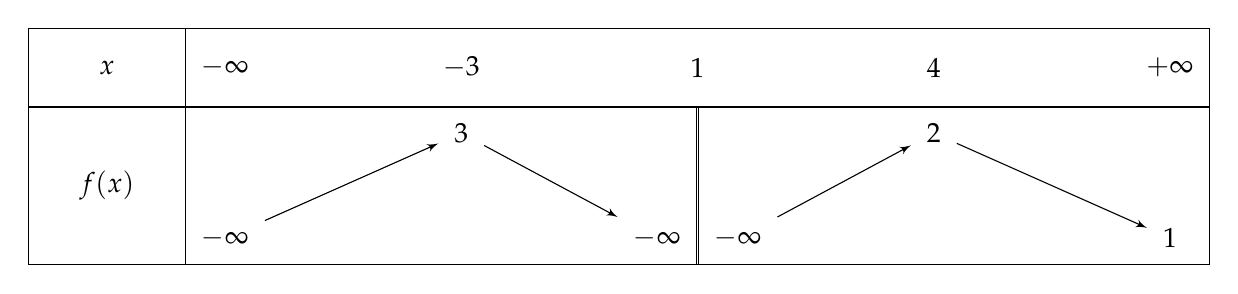
\begin{tikzpicture}
      \tkzTabInit {$x$/1, $f(x)$/2}{$-\infty$, $-3$, $1$, $4$, $+\infty$}
      \tkzTabVar{-/$-\infty$, +/3, -D-/ $-\infty$ /$-\infty$, +/2, -/1}
    \end{tikzpicture}
    On a :
    \begin{itemize}
        \item $f(]-\infty;-3]) = $
        \item $f(]-3;1[) = $
        \item $f(]1;4]) = $
        \item $f(]4;+\infty[) = $
    \end{itemize}
\end{exemple}

\begin{application}
    Soi $f$ la fonction définie sur $\mathbb{R}$ par $f(x) = x^3 - 3x + 1$.\\
    Déterminer les images des intervalles suivants par la fonction $f$ :
    \begin{multicols}{4}
        {\renewcommand{\labelitemi}{}
        \begin{itemize}
            \item $I = ]-\infty; -2]$
            \item $I = [0; 1]$
            \item $I = \left[\displaystyle\frac{1}{3}; +\infty\right[$
            \item $I = [2; 5]$
        \end{itemize}}
    \end{multicols}
\end{application}

\mysubsection{3}{Continuté de la composée de deux fonctions}
\begin{Proposition}
    Soit $f$ une fonction définie sur un intervalle $I$ et $g$ une fonction définie sur un intervalle $J$ tel que $f(I)\subset J$, et soit $a$ un élément de $I$.
    \begin{enumerate}
        \item Si $f$ est continue au point $a$ et $g$ continue au point $f(a)$, alors la fonction $g\circ f$ est continue en $a$.
        \item Si $f$ est continue sur $I$ et $g$ continue sur $J$ alors $g\circ f$ continue sur l'intervalle $I$.
    \end{enumerate}
\end{Proposition}

\begin{exemple}
    \begin{enumerate}
        \item Soit $f$ la fonction définie par : $f(x) = \cos(\displaystyle\frac{1}{\sqrt{x}})$.\\
        On a la fonction $f_1:x\longmapsto\displaystyle\frac{1}{\sqrt{x}}$ est continue sur $]0;+\infty[$ et $f_2:x\longmapsto \cos{x}$ continue sur $\mathbb{R}$ et $f_1(]0;+\infty[)\subset\mathbb{R}$, alors la fonction $f=f_2\circ f_1$ est continue sur $]0;+\infty[$.
        \item Soit $g$ la fonction définie par : $g(x) = \sqrt{1-\sin{x}}$.\\
         On a la fonction $g_1:x\longmapsto 1-\sin{x}$ est continue sur $\mathbb{R}$ et $g_2:x\longmapsto \sqrt{x}$ continue sur $\mathbb{R}^+$ et $g_1(\mathbb{R})\subset\mathbb{R}^+$, alors la fonction $g=g_2\circ g_1$ est continue sur $\mathbb{R}$.
    \end{enumerate}
\end{exemple}

\mysubsection{4}{Théorème des valeurs intermédiaires}
\begin{Proposition}
    Si $f$ une fonction continue sur un intervalle $[a;b]$, alors pour tout réel $\lambda$ compris entre $f(a)$ et $f(b)$, il existe au moins un réel $c\in [a;b]$ tel que $f(c) = \lambda$.

    En d'autre termes : l'équation $f(x) = \lambda$ d'inconnue $x$ admet au moins une solution dans $[a;b]$ pour tout réel $\lambda$ compris entre $f(a)$ et $f(b)$.
\end{Proposition}




&\\
\hline
\end{tabular}

\begin{tabular}{|>{\raggedright\arraybackslash}p{17cm}|>{\centering\arraybackslash}p{0.8cm}|}
\hline


\vspace{1mm}
\begin{Proposition}
    Si $f$ une fonction continue sur un intervalle $[a;b]$ tel que $f(a)\times f(b) < 0$ alors l'équation $f(x) = 0$ admet au moins solution dans l'intervalle $[a;b]$. Si de plus, la fonction $f$ est strictement monotone, cette solution est unique. 
\end{Proposition}
\begin{exemple}
    \begin{enumerate}
        \item Montrons que l'équation $8x^3-6x-1 = 0$ admet une solution dans chacun des intervalles $\left]-1;-\displaystyle\frac{1}{2}\right[$,$\left]-\displaystyle\frac{1}{2};0\right[$, $]0;1[$.
    \end{enumerate}
\end{exemple}
\begin{application}
   \begin{enumerate}
       \item  Montrer que chacune des équations suivantes admet au moins une solution dans l'intevalle $I$ :
            \begin{multicols}{2}
                \begin{enumerate}
                    \item $2\cos{x} - x = 0$  et $I = [0;\pi]$
                    \item $\sin{x} = x^2$ et $I = \left[\displaystyle\frac{\pi}{4};\displaystyle\frac{\pi}{2}\right]$   
                \end{enumerate}
            \end{multicols}
        \item Montrer que chacune des équations suivantes admet une solution unique dans $I$ :
        \begin{multicols}{2}
            \begin{enumerate}
                \item $x^3-6x^2+6 = 0$ et $I = [-2;0]$
                \item $x+\sin{x} = 1$ et $I = \left[0;\displaystyle\frac{\pi}{2}\right]$
            \end{enumerate}
        \end{multicols}
   \end{enumerate}
\end{application}



\mysubsection{5}{Principe de la méthode de Dichotomie}

Soit $f$ une fonction continue sur un segment $[a,b]$ telle que l’équation $f(x) = 0$ admette une solution unique $\alpha$ dans $[a;b]$.\newline

Étape de la méthode : on commence en calculant le milieu du segment $[a,b]$, à savoir $m = \frac{a+b}{2}$, puis son image par $f$, c’est-à-dire $f(m)$.

\begin{itemize}
    \item \textbf{Cas où $f(m) = 0$ :} on a trouvé la solution $r = m$.
    \item \textbf{Cas où $f(m) \neq 0$ :}
        \begin{itemize}
            \item Si $f(a) \cdot f(m) < 0$, la racine est dans $[a,m]$. On reprend la méthode sur cet intervalle en posant $b = m$, puis on continue comme précédemment.
            \item Si $f(m) \cdot f(b) < 0$, la racine est dans $[m,b]$. On reprend la méthode en posant $a = m$, puis on continue comme précédemment.
        \end{itemize}
\end{itemize}
\begin{exemple}
    Soit $f$ la fonction numérique définie par : $f(x) = x^3 + x^2 + x -2$.\\
    La fonction $f$ est continue et strictement croissante sur $[0;1]$ et on a $f(0)\times f(1) < 0$. Donc l'équation $f(x) = 0$ admet une solution unique $\alpha$ tel que $0 < \alpha < 1$. Déterminons un encadrement de $\alpha$ de longeur $0,25$.\\
    Le centre de $[0;1]$ est $\displaystyle\frac{1}{2}$ et on a $f\left(\displaystyle\frac{1}{2}\right) = -\displaystyle\frac{9}{8}$. Donc $f\left(\displaystyle\frac{1}{2}\right)\times f(1) < 0$ et $\displaystyle\frac{1}{2} < \alpha < 1$. (Longeur: $1-\displaystyle\frac{1}{2} = \displaystyle\frac{1}{2}$)\\
    Le centre de $\left[\displaystyle\frac{1}{2};1\right]$ est $\displaystyle\frac{3}{4}$ et on a $f\left(\displaystyle\frac{3}{4}\right) = -\displaystyle\frac{17}{64}.$ Donc $f\left(\displaystyle\frac{3}{4}\right)\times f(1) < 0$ et $\displaystyle\frac{3}{4} < \alpha < 1$. (Longeur : $1 - \displaystyle\frac{3}{4} = \displaystyle\frac{1}{4})$.
    Alors $\displaystyle\frac{3}{4} < \alpha < 1$
\end{exemple}

&\\
\hline


\end{tabular}



\begin{tabular}{|>{\raggedright\arraybackslash}p{17cm}|>{\centering\arraybackslash}p{0.8cm}|}
\hline


\vspace{1mm}
\mysection{Fonction réciproque d'une fonction continue et strictement monotone}\newline
\mysubsection{1}{Théorème de la fonction réciproque}
\begin{Proposition}
    Soit $f$ une fonction continue et strictement monotone sur un itervalle $I$ et soit $J=f(I)$.\\
    pour tout $y\in J$, l'équation $f(x) = y$ admet une solution unique $x$ dans l'intervalle $I$. \\
    La fonction qui à chaque élément $y$ de $J$ associe l'élément unique $x$ de $I$ tel que $f(x) = y$ est appelée \textcolor{red}{la fonction réciproque} de la fonction $f$ et est notée $f^{-1}$.
\end{Proposition}

\textcolor{red}{Remarque : }
\begin{itemize}
    \item Si $f$ est une fonction continue et strictement monotone sur un intervalle $I$ et $J = f(I)$, et si $f^{-1}$ est la fonction réciproque de la fonction $f$, alors :
    $$\begin{cases}
        y=f^{-1}(x) \\
        x\in J
    \end{cases}
    \Longleftrightarrow
    \begin{cases}
        f(y) = x\\
        y\in I
    \end{cases}$$
    \item Pour tout $x\in J$ : $f\circ f^{-1}(x) = x$.
    \item Pour tout $x\in I$ : $f^{-1}\circ f(x) = x$.
\end{itemize}

\begin{exemple}
    Soit $f$ une fonction définie sur l'intervalle $I = [1;+\infty[$ par : 
    $$f(x) = x^2-2x+5$$
    Montrer que $f$ admet une fonction réciproque $f^{-1}$ définie sur un intervalle $J$ à déterminer puis déterminer une expression de $f^{-1}(x)$ pour $x\in J$.
\end{exemple}

\begin{application}
    Dans chacun des cas suivants, montrer que la fonction $f$ admet une fonction réciproque $f^{-1}$ définie sur un intervalle $J$ à déterminer puis déterminer une expression de $f^{-1}(x)$ pour $x\in J$ :
    \begin{multicols}{2}
        \begin{itemize}
            \item $f(x) = 4x - x^2$ et $I = ]-\infty; 2[$
            \item $f(x) = \displaystyle\frac{2x}{x^2+1}$ et $I = [-1;1]$
        \end{itemize}
    \end{multicols}
\end{application}

\mysubsection{2}{Propriétés de la fonction réciproque}
\begin{Proposition}
    Si $f$ est une fonction continue et strictement monotone sur un intervalle $I$, alors :
    \begin{enumerate}
        \item La fonction réciproque $f^{-1}$ est continue sur $f(I)$ et a même sens de variation que la fonction $f$.
        \item Les courbes représentatives de $f$ et de $f^{-1}$, dans un répere orthonormé, sont symétriques par rapport à la première bissectrice (c'est-à-dire par rapport à la droite d'équation $y=x$)
    \end{enumerate}
\end{Proposition}





&\\
\hline

\end{tabular}

\begin{tabular}{|>{\raggedright\arraybackslash}p{17cm}|>{\centering\arraybackslash}p{0.8cm}|}
\hline
\vspace{-5mm}
\begin{center}
    \includegraphics[width=0.4\textwidth]{reciproque.PNG}
\end{center}
\mysection{Fonction racine $n^{\text{iéme}}$ Puissances rationnelle}\newline
\mysubsection{1}{Fonction racine $n^{\text{iéme}}$} \newline
Soit $n$ un entier naturel non nul.\newline
La fonction $f:x\longmapsto x^n$ est continue et strictement croissante sur l'intervalle $\mathbb{R}^+$; donc elle admet une fonction réciproque définie sur l'inetrvalle $f(\mathbb{R}^+) = [f(0);\Lim_{x\to +\infty}f(x)[ = \mathbb{R}^+$.

\begin{Definition}
Soit $n$ un entier naturel non nul.\\
La fonction définie sur $\mathbb{R}^+$ par $x\longmapsto x^n$ admet une foction réciproque définie sur $\mathbb{R}^+$. Cette fonction est appelée \textcolor{red}{fonction racine $n^{\text{iéme}}$} et est notée $\sqrt[n]{x}$ pour tout $x\in\mathbb{R}^+$.\\
Pour tout $x\in\mathbb{R}^+$, $\sqrt[n]{x}$ se lit <<racine $n^{\text{iéme}}$ de $x$>>
\end{Definition}
\begin{Proposition}
    Soit $n$ un entier naturel non nul. Alors :
    \begin{multicols}{3}
        \begin{itemize}
            \item $\sqrt[n]{x} = y \Longleftrightarrow y^n = x$
            \item $\sqrt[n]{x} = \sqrt[n]{y} \Longleftrightarrow x=y$
            \item $\sqrt[n]{x} < \sqrt[n]{y} \Longleftrightarrow x < y$
        \end{itemize}
    \end{multicols}
    \begin{itemize}
        \item Pour tout $x\in\mathbb{R}^+\:\ \sqrt[n]{x^n} = (\sqrt[n]{x})^n = x$
        \item La fonction $x\longmapsto\sqrt[n]{x}$ est continue, strictement croissante sur $\mathbb{R}^+$ et de plus $\Lim_{x\to +\infty}\sqrt[n]{x} = +\infty$.
    \end{itemize}
\end{Proposition}

\textcolor{red}{Remarque : }

Pour tout $x\geq 0$ : $\sqrt[2]{x} = \sqrt{x}$

\begin{Proposition}
    Soient $a$ et $b$ deux réels positifs, et $p$ et $q$ deux entiers naturels supérieurs ou égaux à 2. On a alors les propriétés suivantes :
\begin{multicols}{3}
    \begin{itemize}
        \item $\sqrt[n]{a} \times \sqrt[n]{b} = \sqrt[n]{a \times b}$
        \item $\sqrt[np]{a^p} = \sqrt[n]{a}$
        \item $\sqrt[n]{\displaystyle\frac{1}{a}} = \displaystyle\frac{1}{\sqrt[n]{a}} \quad \text{(avec $a > 0$)}$
        \item $\sqrt[n]{\sqrt[p]{a}} = \sqrt[np]{a}$
        \item $\sqrt[n]{\displaystyle\frac{a}{b}} = \displaystyle\frac{\sqrt[n]{a}}{\sqrt[n]{b}}$
        \item $(\sqrt[n]{a})^p = \sqrt[n]{a^p}$
    \end{itemize}
\end{multicols}
\end{Proposition}
\begin{exemple}
    \begin{enumerate}
        \item Simplifions le nombre : $A = \sqrt{\sqrt{3}} + 2\sqrt[4]{16} - \sqrt[4]{81}$\vspace{-1mm}
        \item Comparons les deux nombres $a=\sqrt[5]{3}$ et $b=\sqrt[4]{4}$\vspace{-1mm}
        \item Résolvons dans $\mathbb{R}$ les équations suivantes : $\sqrt[4]{4-x} = 2$ et $\sqrt[3]{1+x} + \sqrt[3]{1-x} = \sqrt[3]{2}$\vspace{-1mm}
    \end{enumerate}
\end{exemple}
&\\
\hline
\end{tabular}


\begin{tabular}{|>{\raggedright\arraybackslash}p{17cm}|>{\centering\arraybackslash}p{0.8cm}|}
\hline


\vspace{1mm}

\begin{application}
    \begin{enumerate}
        \item Simplifier les nombres suivants : $A = \displaystyle\frac{\sqrt[3]{\sqrt{64}}}{\sqrt{\sqrt[3]{4}}}$ et $B = \displaystyle\frac{\sqrt[4]{9}\times\sqrt{\sqrt[3]{3}\times\sqrt[3]{9}}}{\sqrt[5]{729}\sqrt{\sqrt{\sqrt{3}}}}$
        \item Ranger dans l'ordre croissant les nombres suivants : $\sqrt[12]{9}$; $\sqrt[6]{10}$; $\sqrt[4]{7}$; $\sqrt{3}$
        \item Résoudre dans $\mathbb{R}$ les équations suivantes : 
        
        $16x^4-81 = 0$ \quad;\quad $\sqrt{x} + \sqrt[3]{x} = 12$ \quad;\quad $64 + 125x^3 = 0$ \quad;\quad $(x-1)^3 + 2 = 0$
        \item Résoudre les inéquations suivantes :

        $x^3 - 8 \geq 0$ \quad;\quad $\sqrt[5]{x+2} < 2$ \quad;\quad $\displaystyle\frac{x^3-1}{x^3+8}$
    \end{enumerate}
\end{application}

\begin{Proposition}
Soit $f$ une fonction positive sur un intervalle ouvert $I$ et $a\in I$.
\begin{itemize}
    \item Si $f$ est continue sur $I$ alors la fonction $\sqrt[n]{f}$ est continue sur $I$.
    \item Si $\Lim_{x\to a} f(x) = l$ alors $\Lim_{x\to a}\sqrt[n]{f(x)} = \sqrt[n]{l}$.
    \item Si $\Lim_{x\to a} f(x) = +\infty$ alors $\Lim_{x\to a}\sqrt[n]{f(x)} = +\infty$.
\end{itemize}
\end{Proposition}

\begin{exemple}
Calculons les limites suivantes :
    \begin{enumerate}
        \item $\Lim_{x\to 9}\displaystyle\frac{\sqrt[3]{x-1} - 2}{x-9}$
        \item $\Lim_{x\to +\infty}\sqrt[3]{x^3 + 3x} - 2x$
        \item $\Lim_{x\to +\infty}\sqrt[3]{x^3 + 3x} - x$
        \item $\Lim_{x\to +\infty}\displaystyle\frac{\sqrt{x} - \sqrt[3]{x}}{\sqrt{x} + \sqrt[3]{x}}$
    \end{enumerate}
\end{exemple}
\begin{application}
    \begin{enumerate}
        \item Soit $f$ la fonction définie sur l'intervalle $[-3;+\infty[$ par : 
            $$\begin{cases}
                f(x) = \displaystyle\frac{\sqrt[3]{x+3}-2}{x-5} \text{\quad si } x\neq 5\\
                f(5) = \displaystyle\frac{1}{12}
            \end{cases}$$
            \begin{enumerate}
                \item Montrer que la fonction $f$ est continue sur l'intervalle $[-3;\infty[$.
                \item Calculer la limite $\Lim_{x\to +\infty}f(x)$.
            \end{enumerate}
        \item Calculer les limites suivantes :
        
        $\Lim_{x\to -\infty}\sqrt[3]{1-x^3} + 2x$ \quad;\quad
        $\Lim_{x\to 0}\displaystyle\frac{\sqrt[3]{1+x}-2}{\sin{x}}$ \quad;\quad
        $\Lim_{x\to +\infty}\displaystyle\frac{\sqrt[3]{x+1} - \sqrt{x+1}}{\sqrt[4]{x+1} - \sqrt{x+1}}$ \quad;\quad
    \end{enumerate}
\end{application}
&\\
\hline
\end{tabular}

\begin{tabular}{|>{\raggedright\arraybackslash}p{17cm}|>{\centering\arraybackslash}p{0.8cm}|}
\hline
\vspace{1mm}
\mysubsection{2}{Puissance rationnelle d'un nombre strictement positif}
\begin{Definition}
    Soit $a$ un réel strictement positif et $r$ un nombre rationnel. On pose $r=\displaystyle\frac{p}{q}$ avec $p\in\mathbb{Z}$ et $q\in\mathbb{N}^*$.

    Le nombre $a^r$ est le nombre $\sqrt[q]{a^p}$. Ce nombre est appelé la puissance rationnelle du nombre $a$ d'exposant $r$.
\end{Definition}
\textcolor{red}{Remarque :}

Soit $a$ un réel strictement positif et $n\in\mathbb{N}^*-{1}$.

On a $\sqrt{a}=\sqrt[2]{a} = a^{\frac{1}{2}}$ et $\sqrt{a}=\sqrt[3]{a} = a^{\frac{1}{3}}$. De façon générale, on a l'égalité : $\sqrt[n]{a} = a^{\frac{1}{n}}$.
\begin{Proposition}
    Soit $r$ et $r^{'}$ deux nombres rationnels, et $a$ et $b$ deux réels strictement positifs.

    Alors on a les égalités suivantes :
    
    $a^{r} \times a^{r^{'}} = a^{r+r^{'}}$ \quad;\quad
    $(ab)^r = a^r.b^r$ \quad;\quad
    $(a^r)^{r^{'}} = a^{rr^{'}}$ \quad;\quad
    $a^{-r} = \displaystyle\frac{1}{a^r}$ \quad;\quad
    $\left(\displaystyle\frac{a}{b}\right)^r = \displaystyle\frac{a^r}{b^r}$ \quad;\quad
    $\displaystyle\frac{a^r}{a^{r^{'}}} = a^{r-r^{'}}$
\end{Proposition}

\begin{exemple}
    Simplifions le nombre $A=\displaystyle\frac{\sqrt[4]{32}\times\sqrt[6]{27}\times\sqrt[4]{108}}{\sqrt[4]{6}}$
\end{exemple}

\begin{application}
    \begin{enumerate}
        \item Simplifier les nombres suivants : 
        
        $$A = 27^{\frac{2}{3}} + 16^{\frac{3}{4}} - \displaystyle\frac{2}{\sqrt[4]{8^{-2}}} + \displaystyle\frac{\sqrt[5]{2}}{4^{-\frac{2}{5}}} \text{ et } B = \displaystyle\frac{125^{\frac{2}{9}}\times 625^{\frac{1}{4}}\times 25^{\frac{5}{2}}}{5^{\frac{17}{3}}}$$
        \item Calculer les limites suivantes : 

        $\Lim_{x\to +\infty} \left(x^{\frac{2}{3}} - x^{\frac{1}{2}}\right)$ \quad;\quad
        $\Lim_{x\to +\infty}\frac{x^{\frac{1}{4}} - 2x^{\frac{1}{3}}}{x^{\frac{1}{2}} - 3x}$ \quad;\quad
        $\Lim_{x\to 0^+}\displaystyle\frac{\left(4-x^{\frac{2}{3}}\right)^{\frac{3}{2}} - 8}{x}$
    \end {enumerate}
\end{application}

&\\
\hline
\end{tabular}

\end{document}  